\chapter[Capítulo 3]{Situação e Desenvolvimento do Sistema de Design no TCE-RN}
\label{ch:cap3}

  Tendo em vista o potencial que ferramentas de design e prototipação possuem e a necessidade do Tribunal de Contas do Estado em agilizar o seu processo de desenvolvimento, graças a crescente demanda de novos sistemas para evoluir o serviço prestado não so as suas diretorias como aos entes jurisdicionados foi abordada a possibilidade de o tribunal se interessar pelo o desenvolvimento de um sistema de design.

  Como visto anteriormente um sistema design é um produto, que por sua vez tem a intenção de servir outros produtos, que seriam os sistemas desenvolvidos pela instituição, possibilitar tanto a prototipação rapida como a de alta fidelidade, validar as evoluções feitas em sistemas preexistentes junto aos clientes. Essas são algumas das responsabiliades desse produto.

\section{Situação Atual Do Design no TCE-RN} \label{secao31}
  A história do Tribunal de Contas do Estado começou oficialmente em 12 de janeiro de 1961, data oficial da sua criação \cite{historia_tribunal} O tribunal vem ao longo desses anos evoluindo sempre e gerenciando projetos cadas vez mais complexos, agregando as responsabilidades de fiscalização e divulgação dos pareceres do poder legislativo Municipal. Contudo do ponto de vista do design o TCE-RN avançou pouco nos ultimos anos. Apesar de possuir em suas politicas de desenvolvimento a obrigação da construção de um prototipo que precisa ser validado junto ao cliente para saber se o mesmo tem suas necessidades atendidas essa prototipação atualmente é feita por meio da ferramenta de prototipação Pencil Project (Pencil).

  Em 2019 o TCE iniciou o desenvolvimento de uma nova biblioteca de componentes para construção de interfaces web. Essa biblioteca de é construida em em cima de uma plataforma de desenvolvimento em Javascript chamada Angular, Javascript por sua vez é uma linguagem de Programação que juntamente com as tecnologias HTML (HyperText Markup Language) e CSS (Cascate Style Sheet) representam os 3 pilares do sistema de desenvolvimento web modernos.

  Para a construção do seu front-end, que são sistemas com a qual os usuários interagem diretamente, o tribunal usa tecnologias modernas e em constante evolução, contudo para a prototipação, o Pencil oferece poucas vantagens em relação a maioria das ferramentas citadas no Capítulo \ref{ch:cap2}

  \begin{table*}[!ht]
    \centering
    \caption{Vantagens Figma e Pencil}
    \begin{tabular}{lll}
      
      \rowcolor[HTML]{AAAAAA}
      Caracteristicas             &
      Figma                       &
      Pencil                      \\
      \rowcolor[HTML]{DDDDDD}
      Facil de usar               &
      sim                         &
      sim                         \\
      Colaborativo                &
      sim                         &
      não                         \\
      \rowcolor[HTML]{DDDDDD}
      Animação                    &
      sim                         &
      não                         \\
      Arrastar e soltar           &
      sim                         &
      sim                         \\
      \rowcolor[HTML]{DDDDDD}
      Prototipo de Software       &
      sim                         &
      não                         \\
      Prototipação de Interfaces  &
      sim                         &
      sim                         \\
      \rowcolor[HTML]{DDDDDD}
      Prototipação de UX          &
      sim                         &
      não                         \\
      Teste de Usabilidade        &
      sim                         &
      não                         \\
      \rowcolor[HTML]{DDDDDD}
      Controle de Versao          &
      sim                         &
      não                         \\
    \end{tabular}
    \label{table-figma_vs_pencil}
    \fonte{\cite{figma_vs_pencil}}
  \end{table*}

  O fluxo de trabalho até o momento consistia em copiar um projeto preexistentes e utilizar a maior quantidade possivel de elementos desse documento. No entando como foi dito anteriormente o tribunal passou a evoluir a biblioteca de componentes de front-end dos seus sistemas, e por não possuir um sistema de versionamento o Pencil não é capaz de refletir essas modificações. Tambem não é permitido que o usuario teste a o fluxo da experiência de uso dos sistemas com o usuário. Por esses e outros motivos como demonstrado na Tabela \ref{table-figma_vs_pencil} o Figma foi escolhido como ferramenta de desenvolvimento de sistema design para ser usado neste trabalho, que possui o intuito de trazer uma maneira mais dinamica de criar e testar as interfaces do TCE-RN e permita que a todo sistema possa sofrer mudanças e evoluções mais suavemente.

\section{Reconstrução Do Modelo Existente} \label{secao31}

  Executando uma instância de exemplo da biblioteca e usando o navegador Brave foi possível utilizar uma de suas funcionalidades, o CSS Overview, para inspecionar as caracteristicas do projeto e a situação atual da biblioteca, tornando possivel realizar o levantamento dos diferentes aspectos dos componentes como por exemplo a quantidade de cores presentes nas paginas, onde essas cores eram usadas, quais os códigos hexadecimais referente a cada cor, quantos e quais os breakpoints de tamanho das midias. Um exemplo de inspeção de pagina pode ser encontrao na \ref{fig:tcenglib}

  De posse dos elementos fundamentais que já estavam sendo usados em conjunto com as metricas que os mesmos possuiam o passo seguinte foi a construção dessa instancia atual na ferramenta Figma

  \begin{figure}
    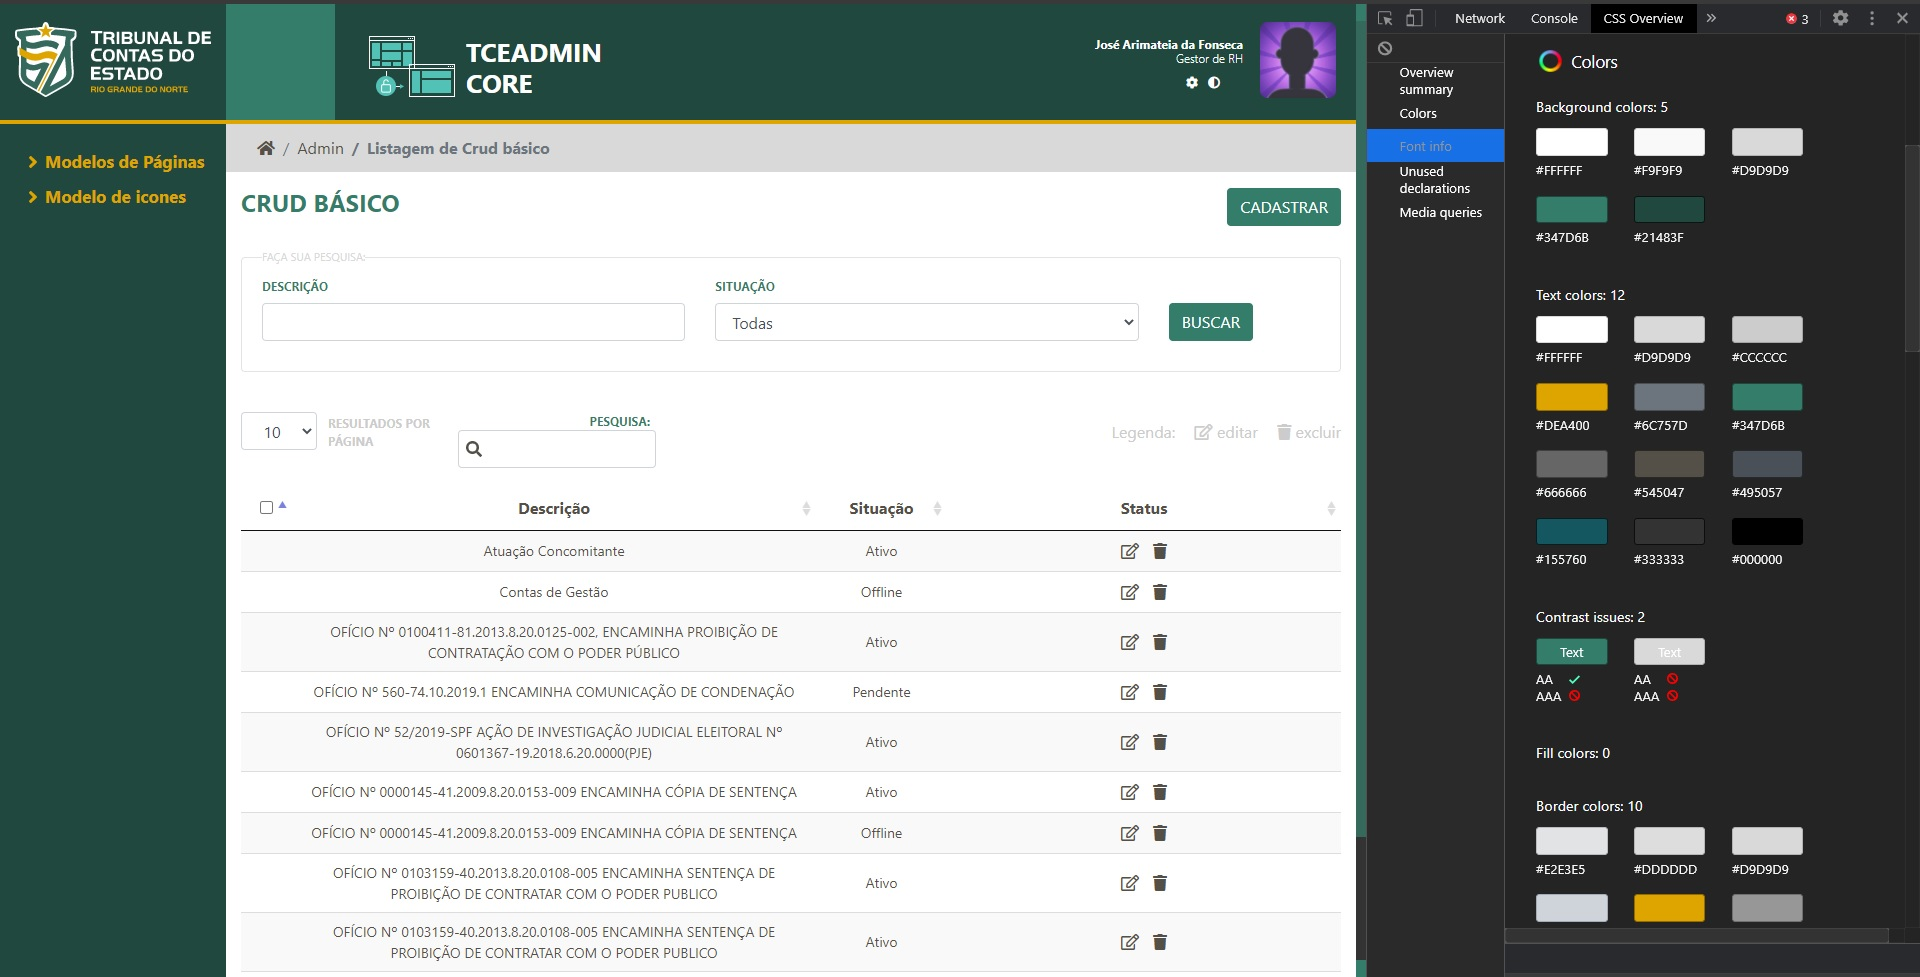
\includegraphics[width=\linewidth]{tce-lib.jpg}
    \caption{Analise da biblioteca de componentes existente no TCE-RN.}
    \label{fig:tcenglib}
  \end{figure}

\section{Problemas Encontrados} \label{secao32}

\section{A Criação De Um Proto Sistema De Design} \label{secao33}

